
%(BEGIN_QUESTION)
% Copyright 2006, Tony R. Kuphaldt, released under the Creative Commons Attribution License (v 1.0)
% This means you may do almost anything with this work of mine, so long as you give me proper credit

En enhet som ligner en pneumatisk trykkregulator er et pneumatisk {\it volumforsterker}-relé:

$$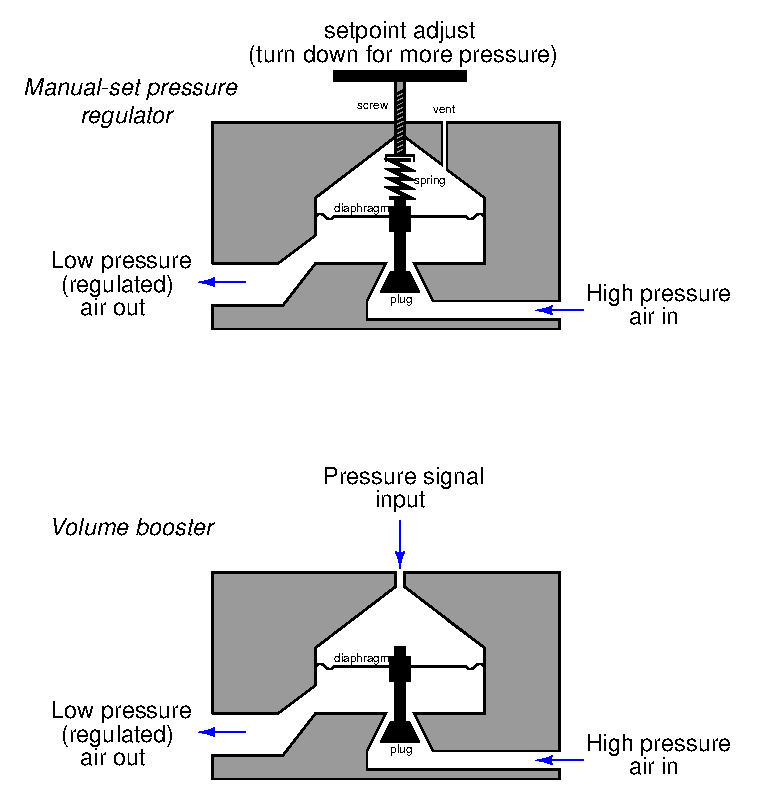
\includegraphics[width=15.5cm]{i00756x01.eps}$$

Formålet med en volumforsterker er å gjenskape samme lufttrykk som inngangssignalet, men med høyere strømningskapasitet enn signalkilden alene klarer å levere.

Forklar hvordan volumforsterkeren fungerer, og hvorfor den kan være nyttig i et pneumatisk instrumenteringssystem som dette:

$$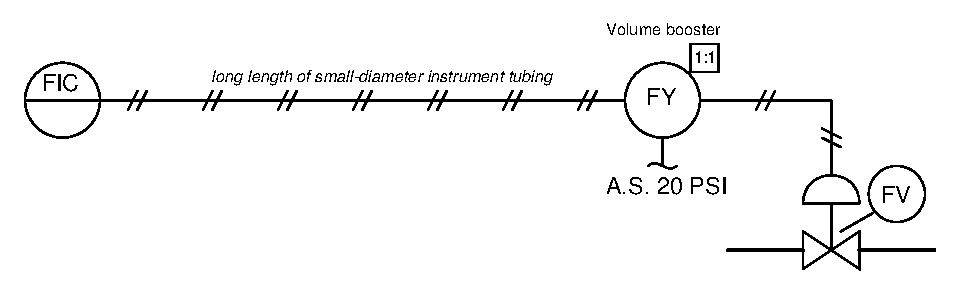
\includegraphics[width=15.5cm]{i00756x02.eps}$$

\underbar{file i00756}
%(END_QUESTION)





%(BEGIN_ANSWER)

En volumforsterker installert i enden av en {\it lang} pneumatisk impulsledning vil forbedre ventilens responstid betydelig ved endringer i regulatorutgangen. Se følgende elektriske analogi for bedre forståelse, der elektrisk ladning tilsvarer pneumatisk volum:

$$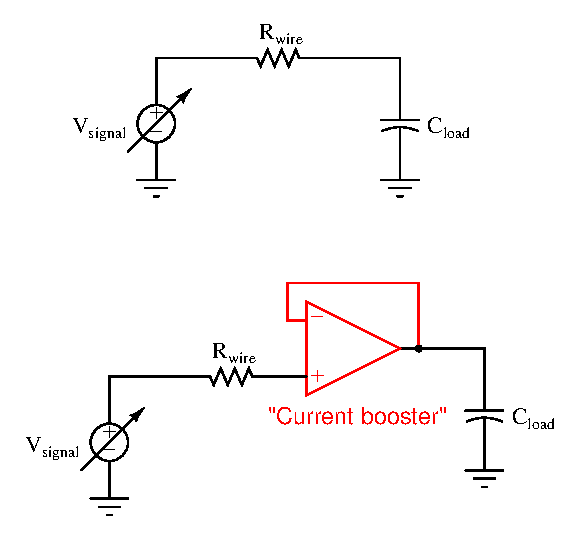
\includegraphics[width=15.5cm]{i00756x03.eps}$$

Den innebygde strømningsmotstanden i impulsledningen (og interne restriksjoner i regulatoren) er analog med elektrisk motstand, mens volumet i ventilaktuatoren er analogt med elektrisk kapasitans. Sammen danner de en ekvivalent RC-tidskonstant.

Når forsterkeren plasseres i enden av ledningen, trenger regulatoren ikke lenger fylle eller tømme et så stort volum (ventilaktuatoren). Det eneste volumet regulatoren nå må styre trykket i, er volumet inne i selve forsterkeren, som er svært lite. Forsterkeren håndterer nå den pneumatiske volumstrømmen aktuatoren trenger, og gjennom en mye kortere (mindre restriktiv) ledningslengde. Dette reduserer systemets «RC-tidskonstant» kraftig og forbedrer responsen.

%(END_ANSWER)





%(BEGIN_NOTES)


%INDEX% Grunnleggende, pneumatikk: trykkforsterker

%(END_NOTES)


